\begin{onehalfspace}
\appendix
\end{onehalfspace}

\chapter{Appendix}

\section{Hollow and Filled Unit Stem Generation Using C++ and GNU Make Utility}

\section*{Source code: \texttt{\textmd{gen\_blockMeshToFile-v8.tex}}}

%\lstset{language=C++,basicstyle=\footnotesize}
\begin{lstlisting}[language=C++,numbers=left,basicstyle={\ttfamily},breaklines=true,showspaces=false]
#include <iostream>
#include <fstream>
#include <ctype.h>
#include <stdio.h>
#include <stdlib.h>
#include <unistd.h>
using namespace std;

int main (int argc, char **argv){
  char		cylinderType, comma ; 
                // hollow (h or H) or filled (f or F)
  double	Rinr = 0.5; 
  double	HLCx = 2.0;
  double	HLCy = 2.0;
  int		nGrZ = 5;
  int		Ninr = 8;
  char		idSp,idX, idY;

  std::ifstream infile("blockMesh.param");
  cylinderType= 'F';
  infile    >> Rinr		// >> comma
	    >> HLSq		// >> comma
	    >> FLCz		// >> comma

  std::cout << "infile  = " << "blockMesh.param" << endl;
  std::cout << "Rinr    = " << Rinr << endl;
  std::cout << "HLSq    = " << HLSq << endl;      
 
 /* omitted */  
  
  /* MERGEPATCHPAIRS */
  outfile <<"mergePatchPairs" <<endl;
  outfile <<"("<<endl;
  outfile <<");"<<endl<<endl;
  outfile <<  "// ******************************** //\n"<<endl;

  outfile.close();
  return 0;}
\end{lstlisting}


\paragraph*{Makefile}

\texttt{}
\begin{lstlisting}[language=make,numbers=left,basicstyle={\ttfamily},breaklines=true]
# Makefile 
version=v8
srcroot=gen_blockMeshToFile-$(version)
cxx=g++
# CXX = c++ compiler
# cxx=icpc
#
gbm:
	$(cxx) $(srcroot).cpp -o $(srcroot).x

hollow:
	cp -f blockMesh.param.default blockMesh.param
	sed -i 's/cylinderType/H/' blockMesh.param $(srcroot).x
	cp blockMeshDict_hollow \
		./stem_hollow/stem_hollow/system/blockMeshDict
	cd ./stem_hollow/stem_hollow && blockMesh

filled:
	cp -f blockMesh.param.default blockMesh.param
	sed -i 's/cylinderType/F/' blockMesh.param $(srcroot).x
	cp blockMeshDict_filled \
		./stem_filled/stem_filled/system/blockMeshDict
	cd ./stem_filled/stem_filled && blockMesh
\end{lstlisting}


\section{MATLAB Script to calculate \texttt{alphaU}}

The following script and associated text files were used to produce
\texttt{AlphaU} datasets for each simulation time step. This MATLAB
script was initially used until modifications were made directly in
the OpenFOAM script to automatically calculate \texttt{alphaU}. As
seen in the README.txt section, there are variables within the matlab
script that will need to be changed depending on the OpenFOAM case
and mesh size.

\section*{AlphaU.m}

\begin{lstlisting}[language=Matlab,numbers=left,basicstyle={\ttfamily},breaklines=true,showspaces=true]
% Create Alpha-U Data Set
% Date Created: September 7, 2019
% Last Updated: September 12, 2019
% Created by: Tyler Tsuchida % Document Name: CreateAlphaU.m
% Location: /home/student/Documents/TylerTsuchida/TylerTsuchidaThesis/
% Description: This script is to create a new dataset, alphaU, for every timestep in an openFOAM simulation
%% Read alpha.water and U values from time-step file
%Some lines beyond this point may need revision
num_point_rows=136500; %number of data points within mesh -- given after U or alphawater header
num_boundary_rows=10500; %number of data points at boundaries -- given after boundary conditions are stated at end of U or alphawater
num_headerlines=22; %number of lines from line 1 of code to line before mes data is written
num_boundarylines=5340528; %number of lines from line 1 of code to line before boundary data is written
folder=3; %the next line of code lists all folders in your simulation directory, to skip invisible folders,
folder=1st time step folder on list
timestep=dir('/media/student/Elements/2019-10-25-Coarse/cavity_cFE_coarse0/cavity_cFE_coarse0'); %insert directory with all timesteps here
%Do not need to edit the code beyond this point
% ...
% ...
end
\end{lstlisting}


\section*{\texttt{alphaU} sections}

\subsection*{alphaU\_Header2.txt}

\begin{lstlisting}[language={C++},numbers=left,basicstyle={\ttfamily}]
object alphaU;
}
//*************************************//
dimensions [0 1 -1 0 0 0 0];
internalField nonuniform List<vector>
5340000
(
\end{lstlisting}


\subsection*{alphaU\_Footer1.txt}

\begin{lstlisting}[language={[GNU]C++},numbers=left,breaklines=true]
) ; 
boundaryField 
{  
 DOWN_btm_F00 { type noSlip; } 
 DOWN_btm_H10 { type noSlip; } 
...        
 DOWN_inn_F36 { type noSlip; }
 DOWN_inn_F46 { type noSlip; }
 merged_LEFT_inn_F40 { type flowRateInletVelocity; volumetricFlowRate constant 0.0075; extrapolateProfile false; value uniform (0.3197619 -0 -0); }
 merged_RGHT_btm_F90 { type pressureInletOutletVelocity; value nonuniform List<vector> 10500 ( 
\end{lstlisting}


\subsection*{alphaU\_Footer2.txt}

\begin{lstlisting}[language={C++},numbers=left,breaklines=true]
) ; }
merged_FRNT_inn_F10 { type noSlip; }
merged_FRNT_btm_F00 { type noSlip; }
merged_BACK_inn_F16 { type noSlip; }
merged_BACK_btm_F06 { type noSlip; }
merged_ATOP_inn_F46 { type zeroGradient; }
merged_ATOP_btm_F96 { type zeroGradient; }
}

// *************************************//
\end{lstlisting}


\section*{README.txt}

\begin{lstlisting}[numbers=left,breaklines=true]
Sources for data files:
alphaU_generator.zip
alphaU_generator:
alphaU_Footer1.txt alphaU_Footer2.txt alphaU_Header2.txt calc_alphaU.m README.txt 
All files listed above must be in the directory of all timestep folders for calc_alphaU.m to run properly. 
Enter directory and other information in calc_alphaU.m as needed to match information of the desired run.
\end{lstlisting}


\section{Symmetry Boundary Condition Shear Calculations}

Along with the shear rate calculations presented in the paper, calculations
were also performed on the fine, medium, and coarse meshes using \texttt{cyclic}
boundary conditions. Also, shear rates of the checkerboard were also
calculated as supplementary information.

\begin{table}[H]
\begin{centering}
\begin{tabular}{|c|r|r|r|r|r|r|}
\hline 
Face Name & $\frac{\partial(\alpha U_{x})}{\partial x}$ & $\frac{\partial(\alpha U_{x})}{\partial y}$ & $\frac{\partial(\alpha U_{x})}{\partial z}$ & $\frac{\partial(\alpha U_{y})}{\partial x}$ & $\frac{\partial(\alpha U_{y})}{\partial y}$ & $\frac{\partial(\alpha U_{y})}{\partial z}$\tabularnewline
\hline 
\hline 
DOWN\_Eab\_merged & 2.64E-02 & 6.91E-09 & 3.90E+00 & -- & -- & --\tabularnewline
\hline 
HOLE\_Eab & -1.49E-02 & 1.12E-07 & -6.66E-11 & -- & -- & --\tabularnewline
\hline 
HOLE\_Eab & -- & -- & -- & -1.01E-07 & 1.81E-02 & 8.54E-11\tabularnewline
\hline 
inlet & 1.07E-03 & 0.00E+00 & 0.00E+00 & -- & -- & --\tabularnewline
\hline 
outlet & 1.07E-03 & 1.13E-09 & -2.57E-04 & -- & -- & --\tabularnewline
\hline 
\end{tabular}\caption{Calculations of shear rate {[}1/s{]} using the fine mesh at time =
3.00s with front and back faces (\texttt{cyclic}).}
\par\end{centering}
\label{tbl:fine_mesh_shear_rate}
\end{table}


\section{Alternative Canopy Orientations}

The following figures shows alternative configurations of 24 stems
embedded on the bed surface. 

\begin{figure}[H]
\begin{centering}
(a)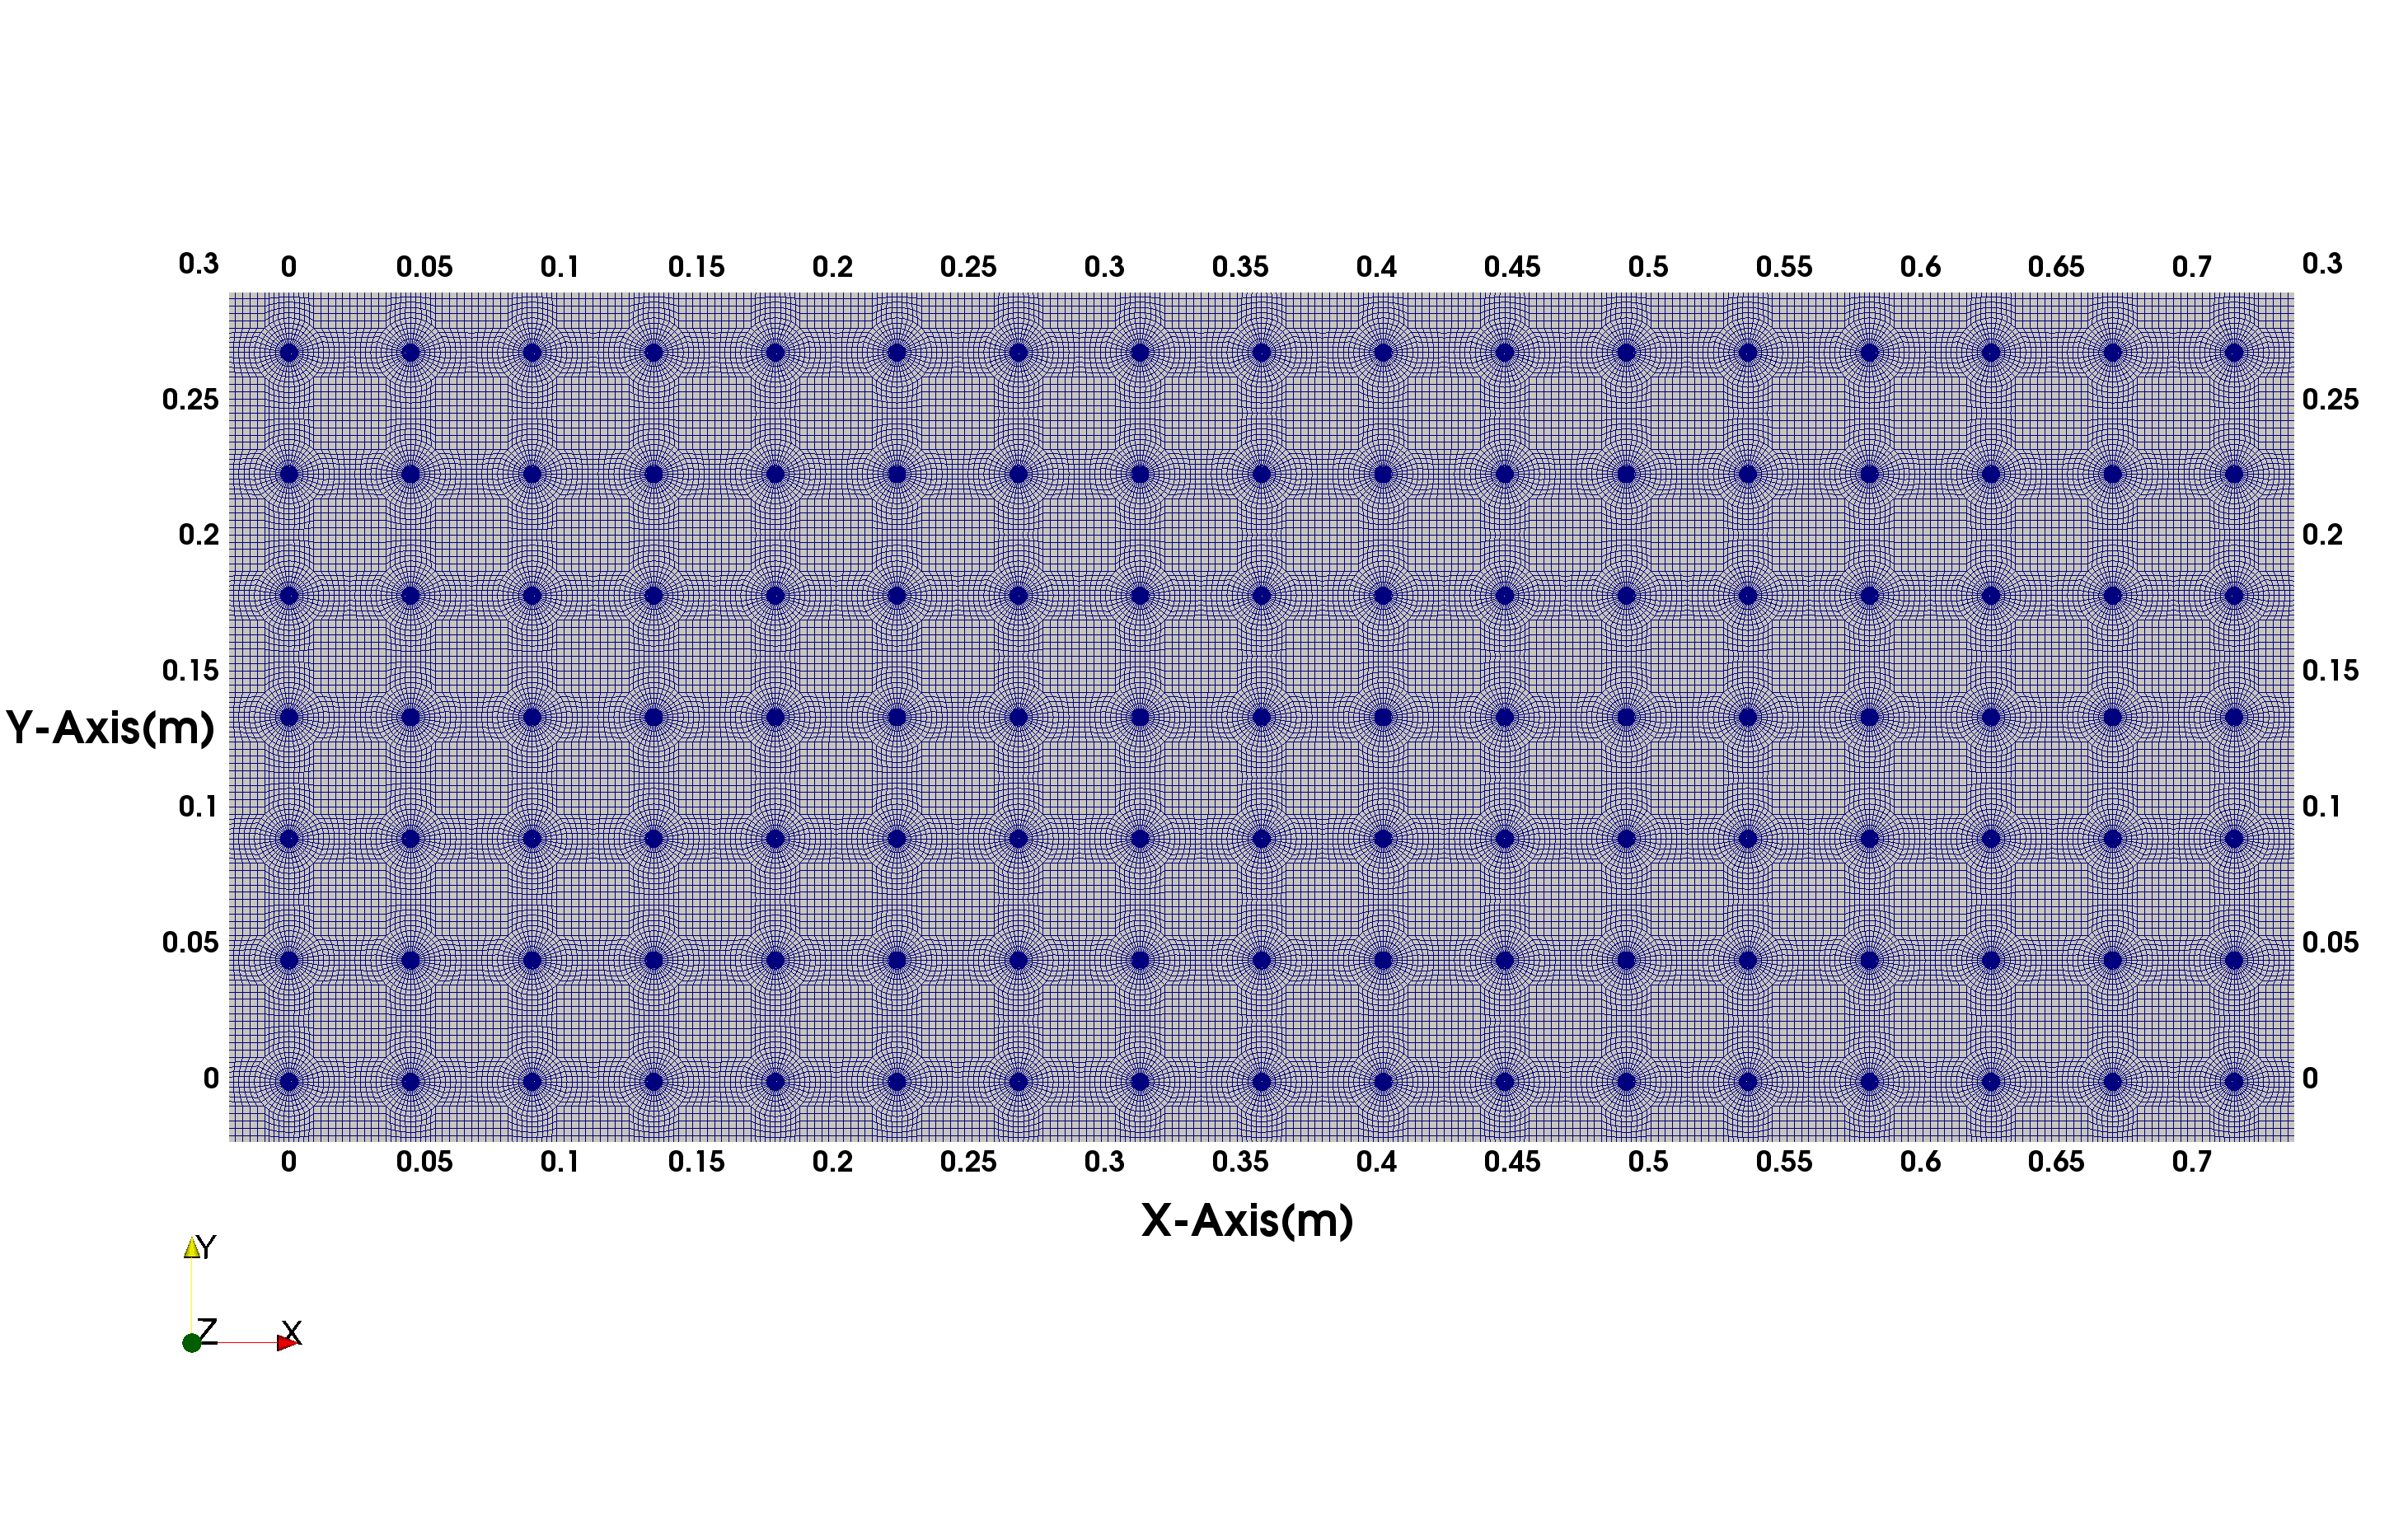
\includegraphics[width=6in]{Figures/0000000_XY}
\par\end{centering}
\begin{centering}
(b)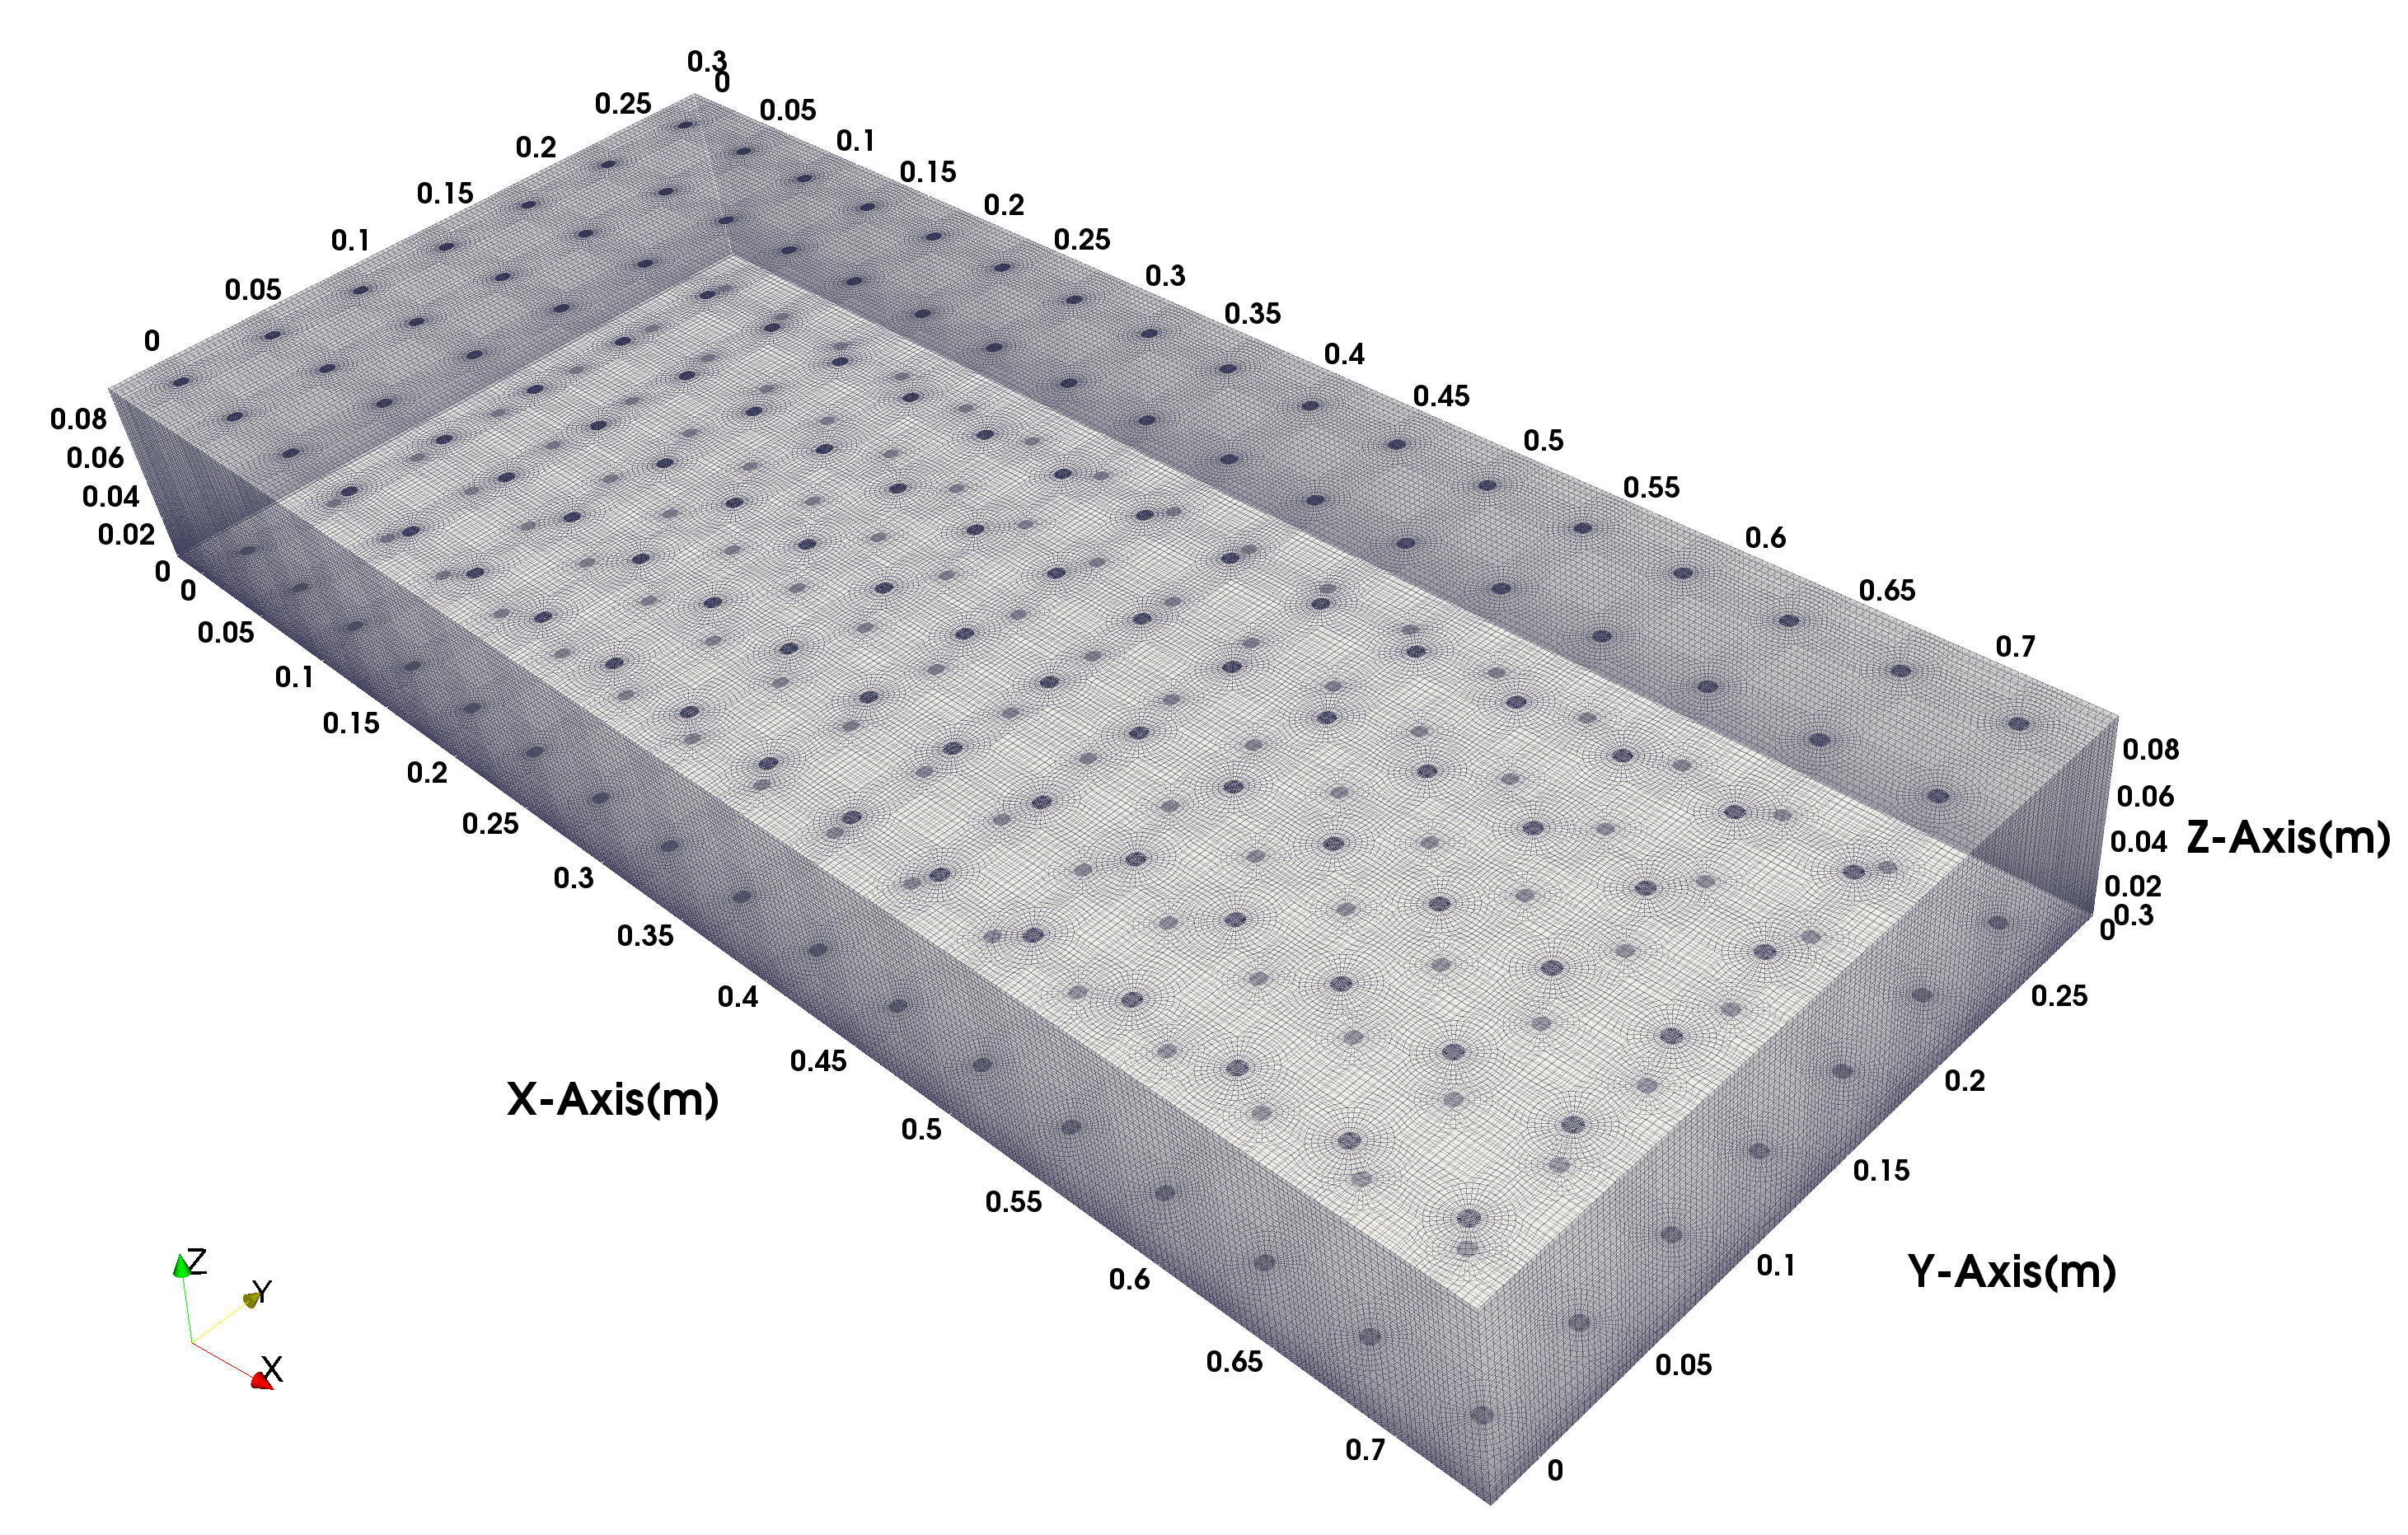
\includegraphics[width=6in]{Figures/0000000_3D}
\par\end{centering}
\caption{0-0-0-0-0-0-0 stem orientation (a)2D and (3) 3D plot.}
\end{figure}

